\chapter{Flowcharts}\label{sec:flowcharts}
%Release Dock
%Release Dock
\begin{figure}[!ht]
\centering
\includegraphics[scale=0.5]{afbeelding/flowcharts/legende.png}
\caption{Flowchart kleurenlegende}
\label{fig:flow:legende}
\end{figure}

\begin{figure}[!ht]
\centering
\includegraphics[scale=0.5]{afbeelding/flowcharts/berichtControleren.png}
\caption{Flowchart voor het ophalen/controleren van berichten}
\label{fig:flow:bericht}
\end{figure}

\begin{figure}[!ht]
\centering
\includegraphics[scale=0.5]{afbeelding/flowcharts/newRelease.png}
\caption{Flowchart van het creëren van een nieuwe release}
\label{fig:flow:release}
\end{figure}

%Field Dock
\begin{figure}[!ht]
\centering
\includegraphics[scale=0.5]{afbeelding/flowcharts/initialisatie.png}
\caption{Flowchart van de initialisatie van een field dock}
\label{fig:flow:init}
\end{figure}

\begin{figure}[!ht]
\centering
\includegraphics[scale=0.5]{afbeelding/flowcharts/agent.png}
\caption{Flowchart van een agent}
\label{fig:flow:agent}
\end{figure}

\begin{figure}[!ht]
\centering
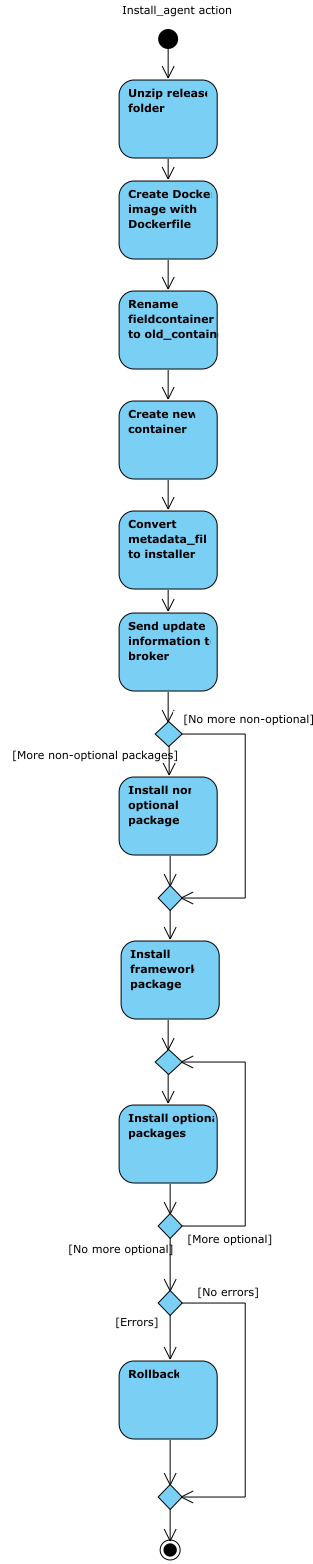
\includegraphics[scale=0.5]{afbeelding/flowcharts/installagent.png}
\caption{Acties van de installagent}
\label{fig:flow:install}
\end{figure}

\begin{figure}[!ht]
\centering
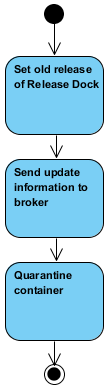
\includegraphics[scale=0.5]{afbeelding/flowcharts/rollback.png}
\caption{Rollback}
\label{fig:flow:rollback}
\end{figure}
